%%%%%%%%%%%%%%%%%%%%%%%%%%%%%%%%%%%%%%%%%
% Masters/Doctoral Thesis 
% LaTeX Template
% Version 2.4 (22/11/16)
%
% This template has been downloaded from:
% http://www.LaTeXTemplates.com
%
% Version 2.x major modifications by:
% Vel (vel@latextemplates.com)
%
% This template is based on a template by:
% Steve Gunn (http://users.ecs.soton.ac.uk/srg/softwaretools/document/templates/)
% Sunil Patel (http://www.sunilpatel.co.uk/thesis-template/)
%
% Template license:
% CC BY-NC-SA 3.0 (http://creativecommons.org/licenses/by-nc-sa/3.0/)
%
%%%%%%%%%%%%%%%%%%%%%%%%%%%%%%%%%%%%%%%%%

%----------------------------------------------------------------------------------------
%	PACKAGES AND OTHER DOCUMENT CONFIGURATIONS
%----------------------------------------------------------------------------------------

\documentclass[
11pt, % The default document font size, options: 10pt, 11pt, 12pt
oneside, % Two side (alternating margins) for binding by default, uncomment to switch to one side
spanish, % ngerman for German
singlespacing, % Single line spacing, alternatives: onehalfspacing or doublespacing
%draft, % Uncomment to enable draft mode (no pictures, no links, overfull hboxes indicated)
%nolistspacing, % If the document is onehalfspacing or doublespacing, uncomment this to set spacing in lists to single
%liststotoc, % Uncomment to add the list of figures/tables/etc to the table of contents
%toctotoc, % Uncomment to add the main table of contents to the table of contents
parskip, % Uncomment to add space between paragraphs
%nohyperref, % Uncomment to not load the hyperref package
headsepline, % Uncomment to get a line under the header
%chapterinoneline, % Uncomment to place the chapter title next to the number on one line
%consistentlayout, % Uncomment to change the layout of the declaration, abstract and acknowledgements pages to match the default layout
]{MastersDoctoralThesis} % The class file specifying the document structure

\usepackage[utf8]{inputenc} % Required for inputting international characters
\usepackage[T1]{fontenc} % Output font encoding for international characters

\usepackage{palatino} % Use the Palatino font by default

\usepackage[backend=biber,style=authoryear,natbib=true]{biblatex} % Use the bibtex backend with the authoryear citation style (which resembles APA)

\addbibresource{bibliografia.bib} % The filename of the bibliography

\usepackage[autostyle=true]{csquotes} % Required to generate language-dependent quotes in the bibliography

%\setlength{\parskip}{2mm}
%----------------------------------------------------------------------------------------
%	MARGIN SETTINGS
%----------------------------------------------------------------------------------------

\geometry{
	paper=a4paper, % Change to letterpaper for US letter
	inner=2.5cm, % Inner margin
	outer=3.8cm, % Outer margin
	bindingoffset=.5cm, % Binding offset
	top=1.5cm, % Top margin
	bottom=1.5cm, % Bottom margin
	%showframe, % Uncomment to show how the type block is set on the page
}

%----------------------------------------------------------------------------------------
%	THESIS INFORMATION
%----------------------------------------------------------------------------------------

\thesistitle{Thesis Title} % Your thesis title, this is used in the title and abstract, print it elsewhere with \ttitle
\supervisor{Dr. James \textsc{Smith}} % Your supervisor's name, this is used in the title page, print it elsewhere with \supname
\examiner{} % Your examiner's name, this is not currently used anywhere in the template, print it elsewhere with \examname
\degree{Doctor of Philosophy} % Your degree name, this is used in the title page and abstract, print it elsewhere with \degreename
\author{John \textsc{Smith}} % Your name, this is used in the title page and abstract, print it elsewhere with \authorname
\addresses{} % Your address, this is not currently used anywhere in the template, print it elsewhere with \addressname

\subject{Biological Sciences} % Your subject area, this is not currently used anywhere in the template, print it elsewhere with \subjectname
\keywords{} % Keywords for your thesis, this is not currently used anywhere in the template, print it elsewhere with \keywordnames
\university{\href{http://www.university.com}{University Name}} % Your university's name and URL, this is used in the title page and abstract, print it elsewhere with \univname
\department{\href{http://department.university.com}{Department or School Name}} % Your department's name and URL, this is used in the title page and abstract, print it elsewhere with \deptname
\group{\href{http://researchgroup.university.com}{Research Group Name}} % Your research group's name and URL, this is used in the title page, print it elsewhere with \groupname
\faculty{\href{http://faculty.university.com}{Faculty Name}} % Your faculty's name and URL, this is used in the title page and abstract, print it elsewhere with \facname

\AtBeginDocument{
\hypersetup{pdftitle=\ttitle} % Set the PDF's title to your title
\hypersetup{pdfauthor=\authorname} % Set the PDF's author to your name
\hypersetup{pdfkeywords=\keywordnames} % Set the PDF's keywords to your keywords
}

\begin{document}

\frontmatter % Use roman page numbering style (i, ii, iii, iv...) for the pre-content pages

\pagestyle{plain} % Default to the plain heading style until the thesis style is called for the body content

%----------------------------------------------------------------------------------------
%	TITLE PAGE
%----------------------------------------------------------------------------------------



%----------------------------------------------------------------------------------------
%	DECLARATION PAGE
%----------------------------------------------------------------------------------------



%----------------------------------------------------------------------------------------
%	QUOTATION PAGE
%----------------------------------------------------------------------------------------



%----------------------------------------------------------------------------------------
%	ABSTRACT PAGE
%----------------------------------------------------------------------------------------



%----------------------------------------------------------------------------------------
%	ACKNOWLEDGEMENTS
%----------------------------------------------------------------------------------------



%----------------------------------------------------------------------------------------
%	LIST OF CONTENTS/FIGURES/TABLES PAGES
%----------------------------------------------------------------------------------------

%\tableofcontents % Prints the main table of contents
%\listoffigures % Prints the list of figures
%\listoftables % Prints the list of tables

%----------------------------------------------------------------------------------------
%	ABBREVIATIONS
%----------------------------------------------------------------------------------------



%----------------------------------------------------------------------------------------
%	PHYSICAL CONSTANTS/OTHER DEFINITIONS
%----------------------------------------------------------------------------------------


%----------------------------------------------------------------------------------------
%	SYMBOLS
%----------------------------------------------------------------------------------------

%----------------------------------------------------------------------------------------
%	DEDICATION
%----------------------------------------------------------------------------------------


%----------------------------------------------------------------------------------------
%	THESIS CONTENT - CHAPTERS
%----------------------------------------------------------------------------------------

\mainmatter % Begin numeric (1,2,3...) page numbering

\pagestyle{thesis} % Return the page headers back to the "thesis" style

% Include the chapters of the thesis as separate files from the Chapters folder
% Uncomment the lines as you write the chapters

% Chapter Template

\chapter{Introducción} % Main chapter title

\label{Chapter1} % Change X to a consecutive number; for referencing this chapter elsewhere, use \ref{ChapterX}

En este primer capítulo se propone dar una visión general del contexto en que se encuadra el proyecto fin de carrera, que es: la visión artificial. Dentro de ésta se abordará el problema al que vamos a hacer frente: La autolocalización visual, o dicho de otro modo, la estimación de la posición y orientación de un sensor con seis grados de libertad (SLAM).

%-----------------------------------
%	SECTION Visión artificial
%-----------------------------------
\section{Visión artificial}

El ser humano no es consciente del proceso neuronal que tiene lugar en nuestro cerebro con el simple hecho de andar o coger un objeto. Se podría decir que tenemos un super ordenador conectado a los órganos sensoriales capaces de recoger muchísima información y procesarla en un tiempo récord.

Desde la antiguedad ya se estuvo pensando en reproducir las habilidades humanas en algún tipo de máquina, la noción de concebir la mente humana como algún tipo de mecanismo no es reciente es referida en célebres filósofos, sin embargo, no es hasta 1950 y con la noción de la computación cuando se introduce la IA (Inteligencia Artificial) por el científico Alan Turing en su artículo \textit{Maquinaria Computacional e Inteligencia} y donde se empieza a coger interés por este campo que será el precursor de una gran cantidad de desarrollos e innovaciones.

Dentro del campo de la inteligencia artificial se puede definir \textbf{visión artificial} como la disciplina científica que incluye métodos para adquirir, procesar y analizar imágenes con el fin de producir información que pueda ser tratada por una máquina ofreciendo soluciones a problemas del mundo real.

Una manera simple de comprender este sistema es basarnos en nuestra propia experiencia. Los humanos usamos nuestros sentidos, especialmente la visión, para comprender el mundo que nos rodea, y la visión artificial busca producir ese mismo efecto en máquinas.

Cada vez son más los dispositivos electrónicos que llevan incorporada al menos una cámara; \textit{smartphones}, ordenadores portátiles, \textit{tablets}, consolas de videojuegos... Debido a la gran cantidad de información que se puede extraer de las imágenes, el bajo coste, el reducido tamaño de las cámaras y el aumento de capacidad de cómputo de los dispositivos, es un área que ha suscitado el interés por los investigadores, ha crecido enormemente en los últimos años y está cogiendo cada vez más fuerza.

% Dispositivos electrónicos
Podemos ver cada vez más como los dispositivos electrónicos disponen de alguna nueva funcionalidad relacionada con el procesamiento de imágenes (Figura~\ref{fig:Face}), como puede ser el reconocimiento facial que incorporan algunos smartphones o tablets para desbloquear el dispositivo o procesado automático de fotos realizadas por la cámara como la que incluye el terminal chino \textbf{Meitu T8} que incorpora un software llamado \textit{AI Beautification} para embellecer las imágenes. \footnote{https://www.cnet.com/products/meitu-t8/preview/}

\begin{figure}[th]
\centering
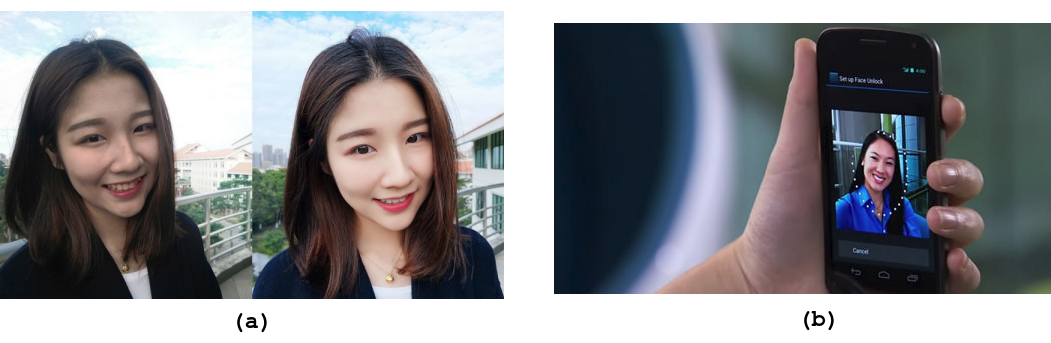
\includegraphics[scale=0.43]{Figures/face.png}
\decoRule
\caption[Embellecimiento de fotos (Meitu T8)]{Embellecimiento de fotos (Meitu T8) (a). Reconocimiento facial (b).}
\label{fig:Face}
\end{figure}

Sin ir más lejos, la reciente aplicación que ha desatado revuelo en las diferentes redes sociales; FaceApp\footnote{https://www.faceapp.com/}. La aplicación disponible tanto para Android e iOS es capaz de añadir sonrisas a las fotos, cambiar de edad o transformar el género de la persona que ha sido fotografiada.

% Medicina
El procesado de imágenes puede llegar a resultar muy útil en otros ámbitos como el de la medicina. Un ejemplo es la radiografía de la Figura~\ref{fig:Medicine} que partiendo de una imágen de muy baja calidad se  pretende  extraer  información  sobre  las  manchas
blancas que aparecen en la misma.

\begin{figure}[th]
\centering
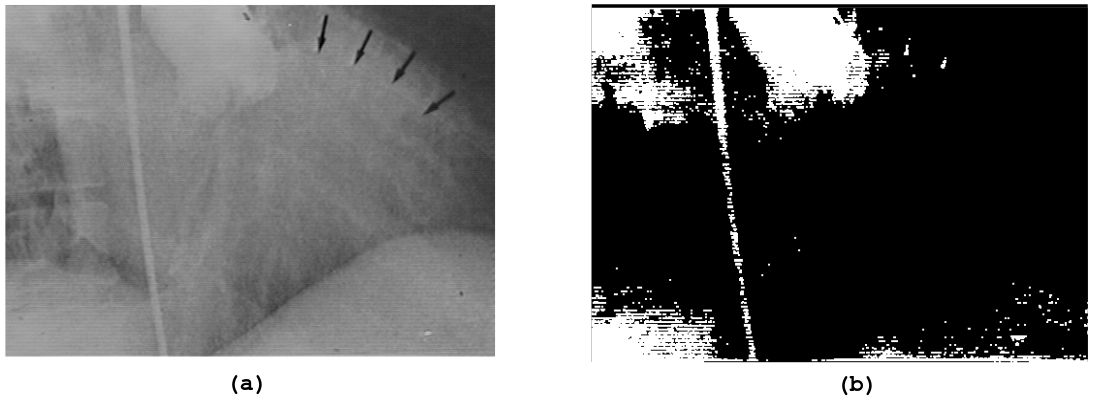
\includegraphics[scale=0.4]{Figures/medicine.png}
\decoRule
\caption[Aplicaciones de radiografía en medicina]{Radiografía inicial, con los puntos a analizar (a), imagen final procesada (b).}
\label{fig:Medicine}
\end{figure}

% Industria
Son numerosas las aplicaciones de visión industrial relacionadas con el entorno de la alimentación. Permiten automatizar el control de calidad para tomar la decisión si un determinado producto cumple el estándar de calidad o no. Un ejemplo es el sistema \textbf{EggInspector}\footnote{http://www.moba.net/page/es/Grading/Moba-Grader-Options/Detection-Systems/Egg-inspector} por la empresa Moba que se utiliza para clasificar huevos de gallina de forma automática. El sistema está compuesto por 6 cámaras suspendidas por encima de la cinta transportadora que con unos complejos algoritmos no solo pueden comprobar si los huevos están rotos o sucios, sino que son capaces de determinar el tipo de rotura y suciedad, una vez determinada la calidad, los que no corresponden a los estándares mínimos, son separados de la línea por un robot.

Siguiendo en la línea de la industria la inspección de embalajes se ha incrementado enormemente con la automatización del proceso y la visión artificial facilitando tareas como la detección del correcto nivel de llenado, verificación de tapones, control de calidad de sellado, lectura de óptica de caracteres (OCR), códigos de barras, verificación de posición, calidad de impresión de las equiquetas, conteo de productos en cajas o \textit{palets}. Algunas de las aplicaciones típicas de la industria del \textit{packaging} están representadas en la Figura~\ref{fig:Industry}.

\begin{figure}[th]
\centering
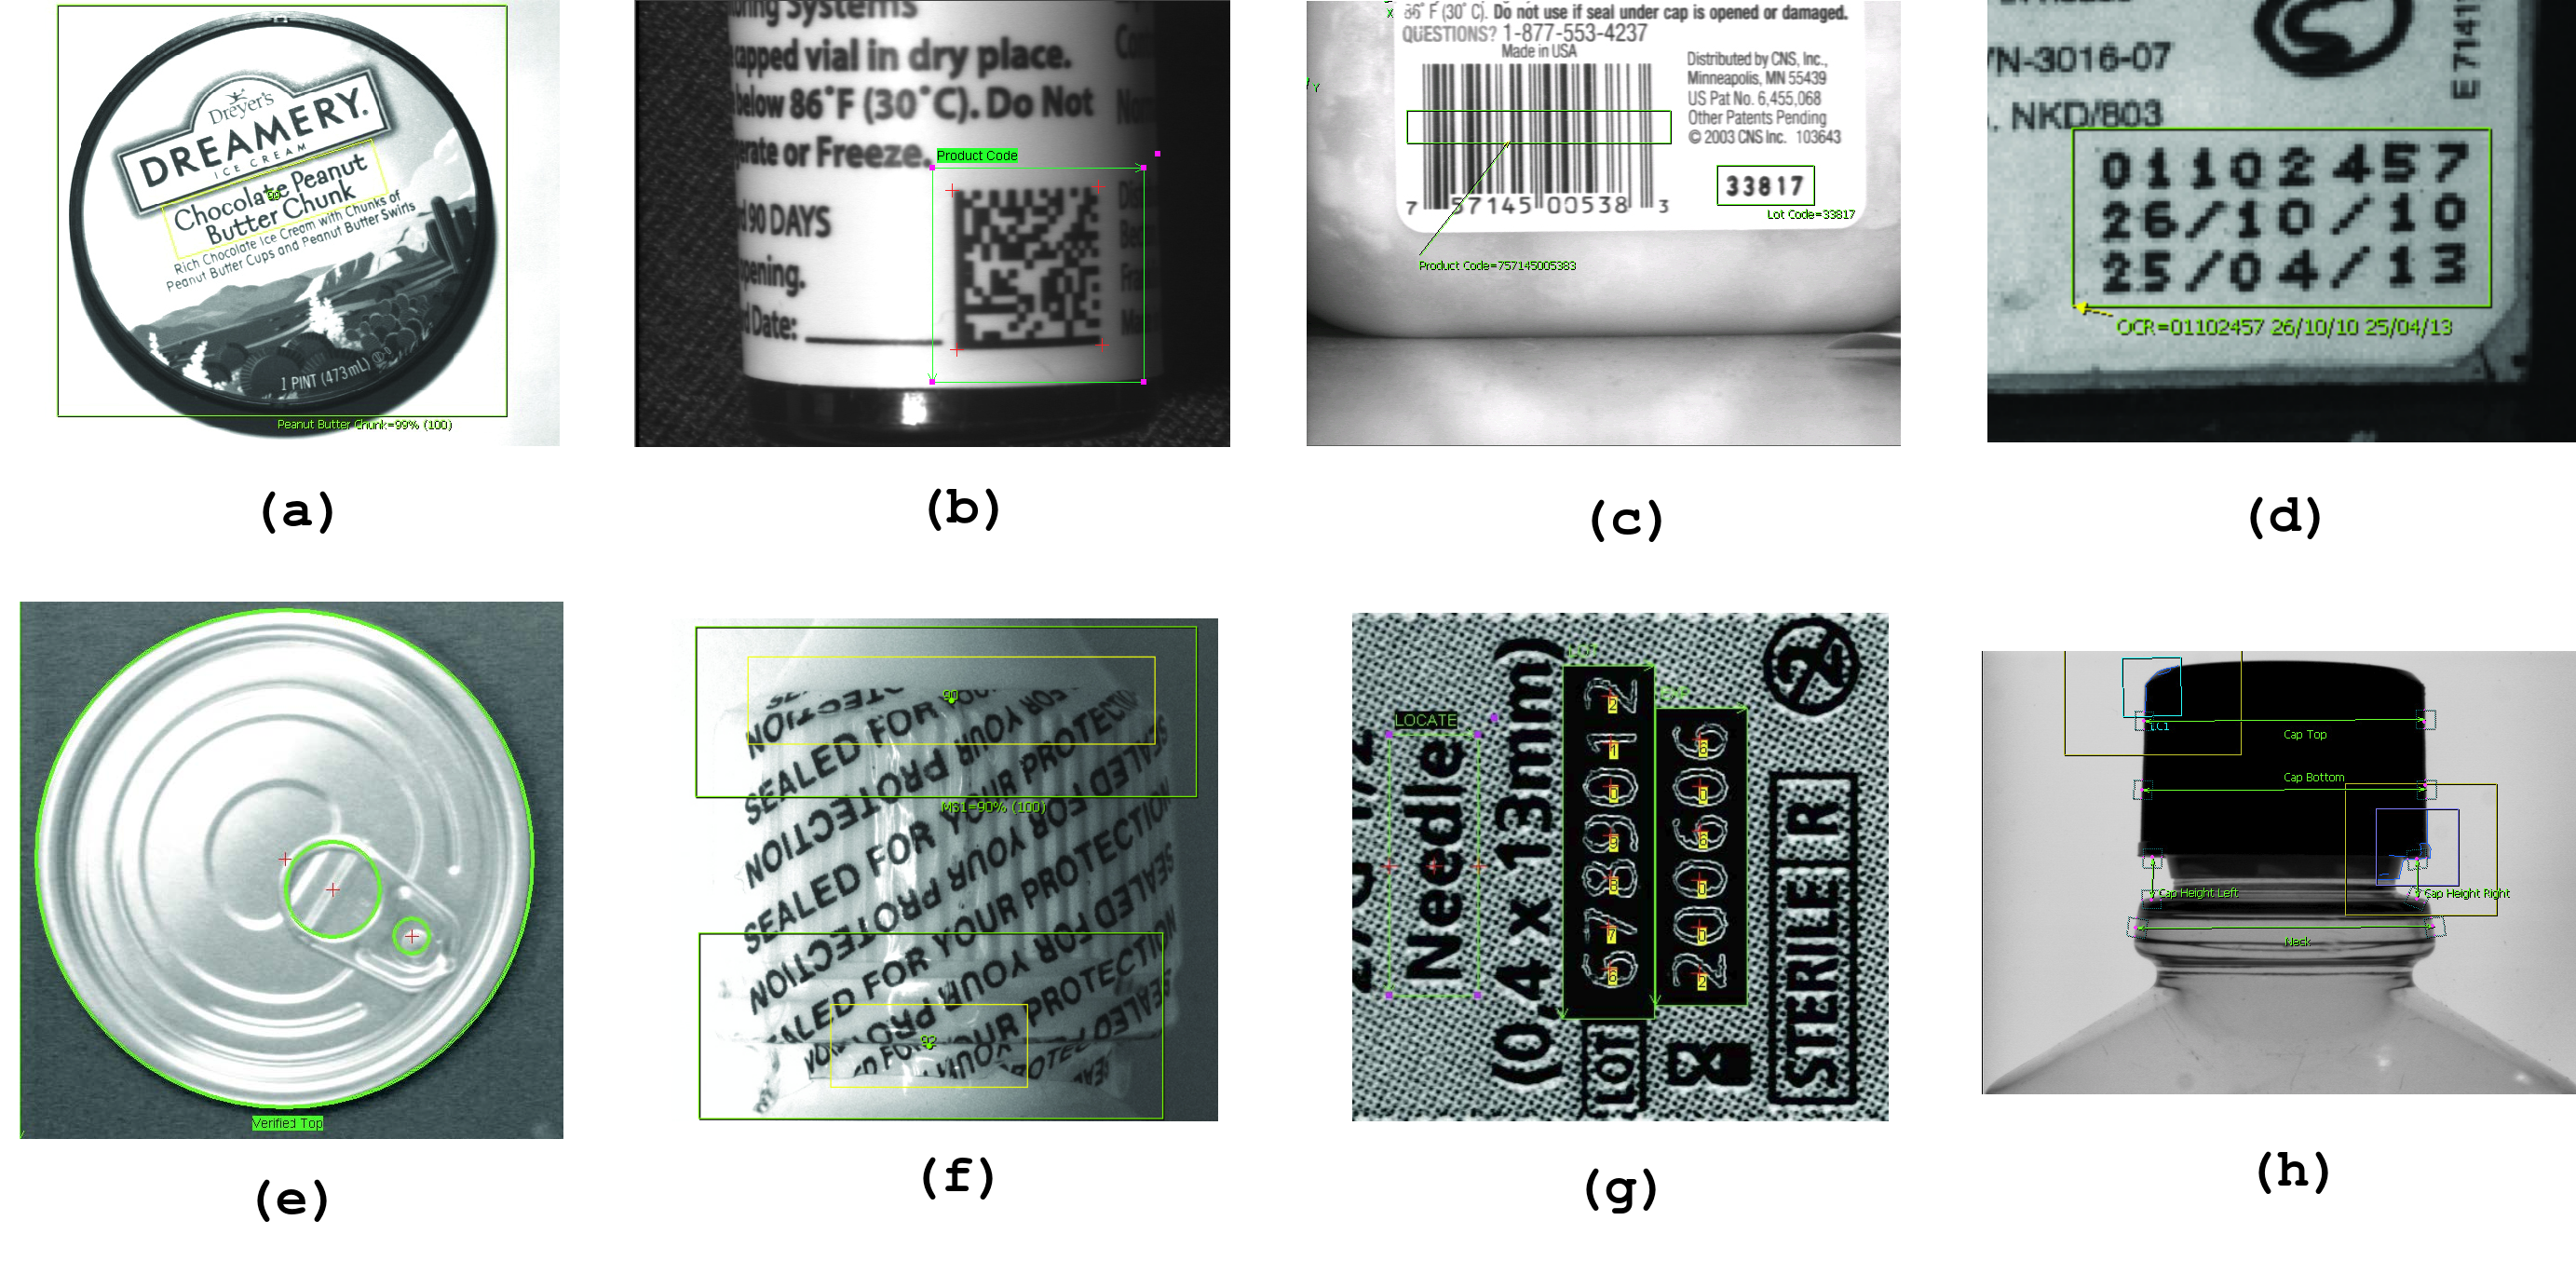
\includegraphics[scale=0.17]{Figures/industry.png}
\decoRule
\caption[Visión en la industria]{Presencia, aplicación e integridad de etiquetas (a), códigos 2D (b), códigos de barras (c), validación de lote, fecha y código (d), orientación de piezas montadas (e), correcto sellado (f), calidad de impresión (g), presencia y cierre de tapones (h). }
\label{fig:Industry}
\end{figure}

% Deportes
En los deportes quizás la aplicación más conocida sea el Ojo de Halcón (Figura~\ref{fig:Ojohalcon}), que se utiliza en los torneos de tenis de alto nivel para determinar la trayectoria de la pelota y saber si entró o no en el campo contrario. Además la visión artificial se usa en numerosos deportes sobretodo en estudios estadísticos post-partido para averiguar el tiempo de posesión del balón en los partidos de fútbol o los kilómetros recorridos por cada jugador en el terreno de juego, entre muchos otros.

\begin{figure}[th]
\centering
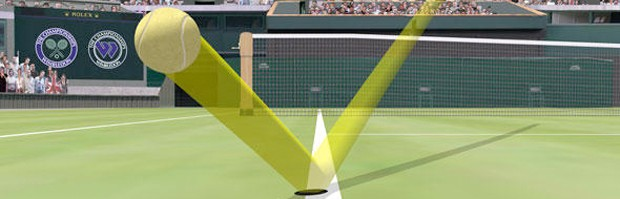
\includegraphics[scale=0.6]{Figures/ojohalcon.jpg}
\decoRule
\caption[Ojo de halcón]{Ojo de Halcón en tenis}
\label{fig:Ojohalcon}
\end{figure}

Actualmente se pueden encontrar sistemas de asistencia y seguridad en los vehículos más modernos como; sistemas de frenado automático de emergencia, asistente de mantenimiento de carril o aparcado automático. Aunque estos sistemas se entienden como asistentes o ayudas a la condución, el conductor sigue tomando la gran responsabilidad de la navegación.

La empresa israelí \textbf{Mobileye}\footnote{https://www.mobileye.com/} presentará su primer modelo de vehículo completamente autónomo, junto a Intel y BMW, en 2021. El cerebro de la máquina se basa en un sensor, que identifica lo que ocurre a su alrededor al instante: los carriles, las señales de tráfico, otros automóviles, motos, bicicletas e incluso a los peatones. En la Figura~\ref{fig:Car} se puede ver una captura de la vista del coche antes de parar en un semáforo.

\begin{figure}[th]
\centering
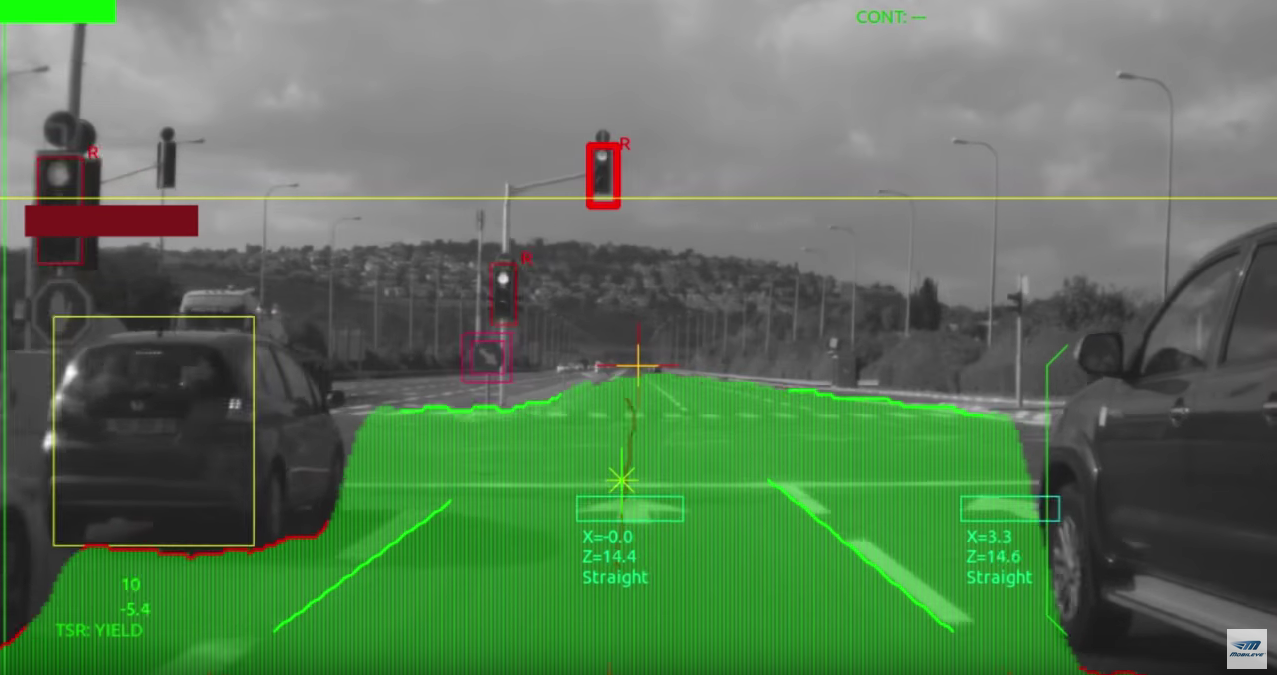
\includegraphics[scale=0.3]{Figures/car.png}
\decoRule
\caption[Visión para la autoconducción]{Vista del coche antes de parar en un semáforo.}
\label{fig:Car}
\end{figure}


\section{Autolocalización visual}
Dentro de la visión artificial se encuentra la autolocalización visual consiste en conocer la localización 3D de la cámara en todo momento solamente con las imágenes capturadas y sin disponer de ninguna información extra. Debido al gran abanico de posibilidades que abre resolver este problema, se sitúa en uno de los retos más importantes dentro del campo de la robótica.

%coches
Esta técnica se plantea en los sistemas de navegación automáticos naúticos, terrestres y aéreos. Actualmente numerosas empresas están invirtiendo en este tipo de sistemas en el que apuestan por una navegación total o parcialmente autónoma.

La autolocalización visual es una técnica que permite aplicaciones de realidad aumentada, que es el término que se usa para definir una visión directa o indirecta de un entorno físico del mundo real, cuyos elementos se combinan con elementos virtuales generados por ordenador para la creación de una realidad mixta en tiempo real.

Aunque se ha popularizado con el juego de \textbf{Pokémon Go}\footnote{http://www.pokemongo.com/es-es/}, cada vez son más los gigantes tecnológicos que se interesan por ella. La empresa sueca Ikea ya cuenta con una aplicación móvil que permite ver su catálogo en realidad aumentada (Figura~\ref{fig:Ikea}).

\begin{figure}[th]
\centering
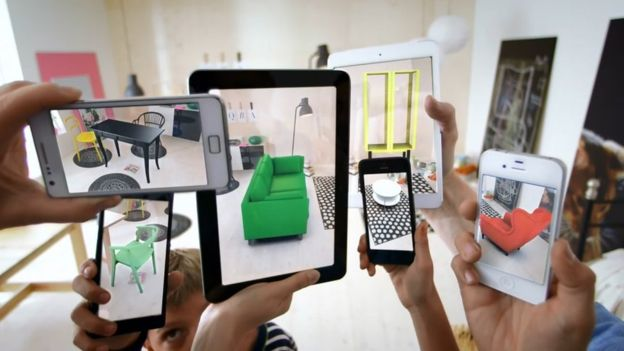
\includegraphics[scale=0.7]{Figures/ikea.jpg}
\decoRule
\caption[Ikea con realidad aumentada]{Catálogo Ikea con realidad aumentada.}
\label{fig:Ikea}
\end{figure}

Puesto que la realidad virtual es una experiencia ficticia, tiene gran potencial en el mundo de los videojuegos. Pero no es el único. También puede tener aplicaciones en medicina, la industria del cine, la moda, los deportes o la publicidad.

%-----------------------------------
%	SECTION Técnicas de autolocalización
%-----------------------------------
%\section{Técnicas de autolocalización visual}

Las técnicas de autolocalización ha suscitado gran interés por los investigadores en los últimos años. El problema ha sido abordado por dos comunidades distintas, por un lado la de visión artificial que denominó al problema como \textbf{structure from motion (SfM)}, donde la información es procesada por lotes, capaz de representar un objeto 2D a 3D con solo unas cuantas imágenes desde diferentes puntos de vista. Y por otro lado la comunidad robótica denominó al problema \textbf{SLAM} (\textit{Simultaneous Localization and Mapping}) que trata de resolver el problema de una manera más compleja adaptando el funcionamiento de los sistemas en tiempo real.

%-----------------------------------
%	SUBSECTION Structure from Motion
%-----------------------------------
\subsection{Structure from Motion (SfM)}

Las técnicas SfM se analizan generalmente de forma \textit{offline}, las escenas se graban a través de un conjunto de imágenes y luego se procesan, lo que permite realizar optimizaciones para el cálculo de la trayectoria, como por ejemplo el ajuste de haces.

Existen aplicaciones comerciales que utilizan estas técnicas como es el caso de la aplicación PhotoTourism \parencite{Reference2} desarrollada por Microsoft. Que consiste en el cálculo de la posición 3D en la que fueron captadas las imágenes, por ejemplo de un monumento, para después extraer el modelo 3D con el que el usuario puede interactuar libremente (Figura~\ref{fig:Tourism}).

\begin{figure}[th]
\centering
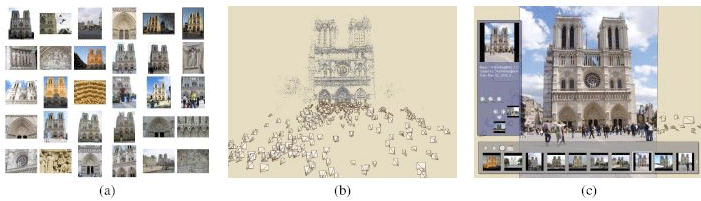
\includegraphics[scale=0.57]{Figures/phototourism.png}
\decoRule
\caption[PhotoTourism]{PhotoTourism: Se recogen una gran colección de imágenes (a), se reconstruyen los puntos 3D y los puntos de vista (b), por último la interfaz permite al usuario interactuar moviendose a través del espacio 3D mediante la transición entre fotografías.}
\label{fig:Tourism}
\end{figure}

%-----------------------------------
%	SUBSECTION Visual SLAM
%-----------------------------------
\subsection{Visual SLAM}

En el problema conocido como \textit{Simultaneous Localization and Mapping} (SLAM) busca resolver los problemas que plantea colocar un robot móvil en un entorno y una posición desconocidas, y que él mismo se encuentre capaz de construir incrementalmente un mapa de su entorno consistente y a la vez utilizar dicho mapa para determinar su propia localización.

La solución a este problema conseguiría hacer sistemas de robots completamente autónomos que junto con un mecanismo de navegación el sistema se encontrara con la capacidad para saber a dónde desplazarse, ser capaz de encontrar obstáculos y reaccionar ante ellos de manera inteligente.

La resolución al problema SLAM visual ha suscitado un gran interés en el campo de la robótica y se han propuesto muchas técnicas y algoritmos para dar solucón al problema, como es el caso del artículo de \cite{Reference1}. Y aunque algunas de ellas han obtenido buenos resultados en la práctica siguen surgiendo problemas a la hora de buscar el método más rápido o el que genere un mejor resultado con menos índice de fallo. La búsqueda de algoritmos y métodos que resuelvan completamente estos problemas sigue siendo una tarea pendiente.

Uno de los trabajos más importantes en el ámbito es el de monoSLAM de Davison\footnote{http://www.doc.ic.ac.uk/\textasciitilde ajd/} \parencite{Reference5} que propone resolver este problema con una única cámara RGB como sensor y realizar el mapeado y la localización simultáneamente. El algoritmo propuesto por Davison utiliza un filtro extendido de Kalman para estimar la posición y la orientación de la cámara, así como la posición de una serie de puntos en el espacio 3D. Para determinar la posición inicial de la cámara es necesario a priori dotar de información con la posición 3D de por lo menos 3 puntos. Después el algoritmo es capaz de situar la cámara en el espacio tridimensional y de generar nuevos puntos para crear el mapa y servir como apoyo a la propia localización de la cámara. En la Figura~\ref{fig:Monoslam} se pueden ver unas capturas de pantalla sobre uno de los experimientos realizados.

\begin{figure}[th]
\centering
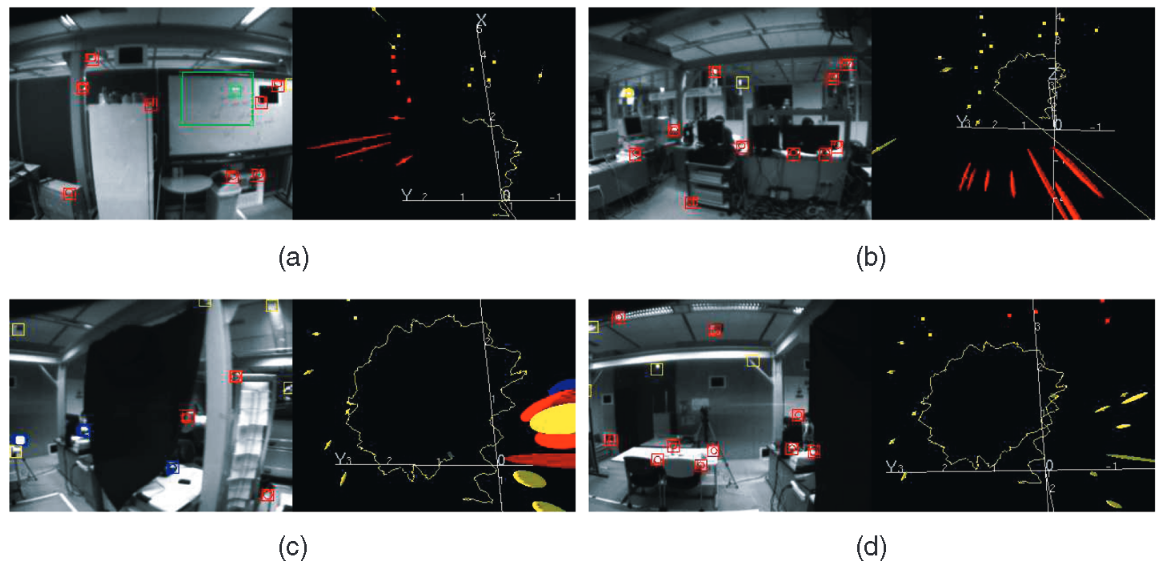
\includegraphics[scale=0.35]{Figures/monoslam.png}
\decoRule
\caption[MonoSLAM]{MonoSLAM: Un robot humanoide camina en una trayectoria circular de radio 0.75m. La estela amarilla muestra la trayectoria estimada del robot, y las elipses muestran los errores de localización.}
\label{fig:Monoslam}
\end{figure}

Es importante destacar también la trascendencia que ha tenido el trabajo PTAM \parencite{Reference6} que viene a solucionar uno de los principales problemas que tienen los algoritmos monoSLAM; el tiempo de cómputo, ya que aumenta exponencialmente con el número de puntos (Figura~\ref{fig:Ptam}). Para ello se aborda el problema separando el mapeado de la localización, de tal modo que solo la localización deba funcionar en tiempo real, dejando así que el mapeado trabaje de una manera asíncrona. Este algoritmo parte de la idea de que solo la localización es necesaria que funcione en tiempo real. PTAM hace uso de \textit{keyframes}, es decir, fotogramas clave que se utilizan tanto para la localización como para el mapeado y también de una técnica de optimización mediante ajuste de haces, como en SfM.

\begin{figure}[th]
\centering
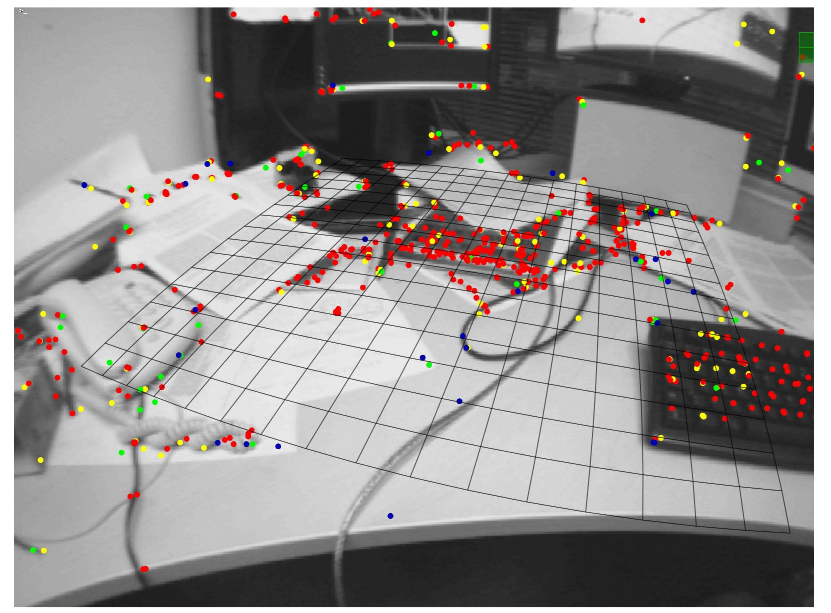
\includegraphics[scale=0.4]{Figures/ptam.png}
\decoRule
\caption[PTAM]{PTAM: Funcionamiento típico del sistema sobre un escritorio.}
\label{fig:Ptam}
\end{figure}

\subsection{Odometría visual}

Dentro de las familias de técnicas pertenecientes a Visual SLAM se encuentra la de odometría visual, que es la que abordaremos en este trabajo. Consiste en la estimación del movimiento 3D de la cámara en tiempo real. Es decir, el cálculo de la rotación y traslación de la cámara a partir de imágenes consecutivas. Se trata de una técnica incremental ya que se basa en la posición anterior para calcular la nueva.

En este tipo de algoritmos se suelen utilizar técnicas de extracción de puntos de interés, cálculos de descriptores y algoritmos para el emparejamiento. Normalmente el proceso es: una vez calculados los puntos emparejados se calcula la matriz fundamental o esencial y descomponerlas mediante SVD para obtener la matriz de rotación y traslación (RT) (\cite{Reference3}. \cite{Reference4}).

%-----------------------------------
%	SECTION Autolocalización visual en del Laboratorio de Robótica URJC
%-----------------------------------
\section{Autolocalización visual en el laboratorio de robótica URJC}

En esta sección se recapitulan algunos de los proyectos, dentro del campo de la autolocalización, realizados por compañeros en el laboratorio de robótica de la Universidad Rey Juan Carlos.

En el proyecto de Luis Miguel López Ramos \parencite{ref1} se diseña y programa un algoritmo que estima en tiempo real la posición y orientación de una cámara móvil autónoma en un entorno estático, utilizando exclusivamente las imágenes obtenidas por la cámara. El algoritmo se valida experimentalmente haciendo uso de una cámara de videoconferencia real y en condiciones de laboratorio.

Se calcula, por tanto, la trayectoria realizada y se muestra en una ventana de gráficos OpenGL junto con un modelo de la cámara y las regiones de confianza de los puntos de referencia. (Figura~\ref{fig:ramos}).

\begin{figure}[th]
\centering
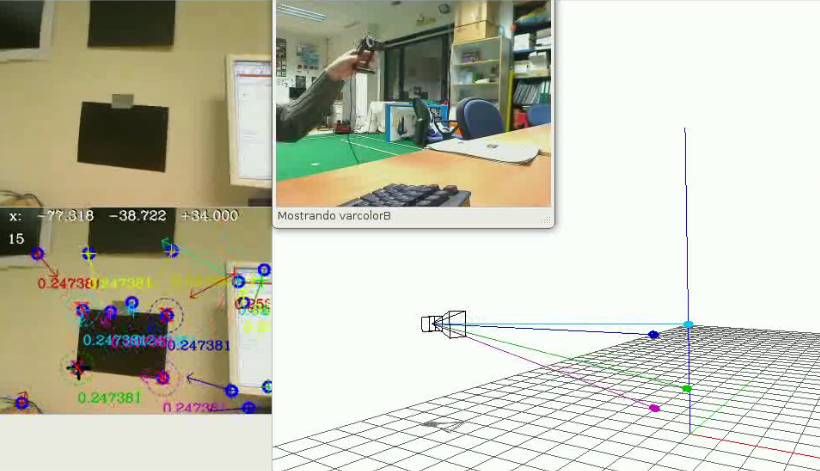
\includegraphics[scale=0.463]{Figures/cap-ramos.png}
\decoRule
\caption[Captura de pantalla, PFC de Luis Miguel]{Captura de pantalla del componente desarrollado por Luis Miguel.}
\label{fig:ramos}
\end{figure}

Eduardo Perdices García \parencite{ref3} propone en su trabajo de fin de master un proyecto de robótica autónoma. Dentro de este área se desarrolla la \textbf{RoboCup}, donde un grupo de robots autónomos deben jugar al fútbol de forma cooperativa variando su comportamiento en función de su posición en el campo, por lo que es muy importante que el robot conozca su posición en todo momento. A partir de los distintos sensores con los que cuenta el robot, como sensores de ultrasonido, sensores laser o cámaras, el robot tiene que estimar su posición en el mundo que le rodea.

En este proyecto se han desarrollado las técnicas necesarias para autolocalizar a un robot humanoide Nao\footnote{http://aliverobots.com/nao/} dentro de un campo de fútbol de la plataforma estándar de la RoboCup utilizando solo una cámara como sensor externo.

Alberto Lopéz-Cerón Pinilla \parencite{ref2} caracteriza un algoritmo de autolocalización visual basado en marcadores. Para ello, desarrolla un componente que a partir de la detección de balizas visuales en una imagen, estima la posición y la orientación de la cámara, mostrando el modelo de la cámara resultante en una ventana OpenGL.

El algoritmo se ha validado experimentalmente realizando estudios de precisión en dos ámbitos: por un lado el de entorno simulado de Gazebo, haciendo uso de un modelo robótico virtual con sus cámaras asociadas, y por otro en un entorno real con una cámara de videoconferencia (Figura~\ref{fig:ceron}).

\begin{figure}[th]
\centering
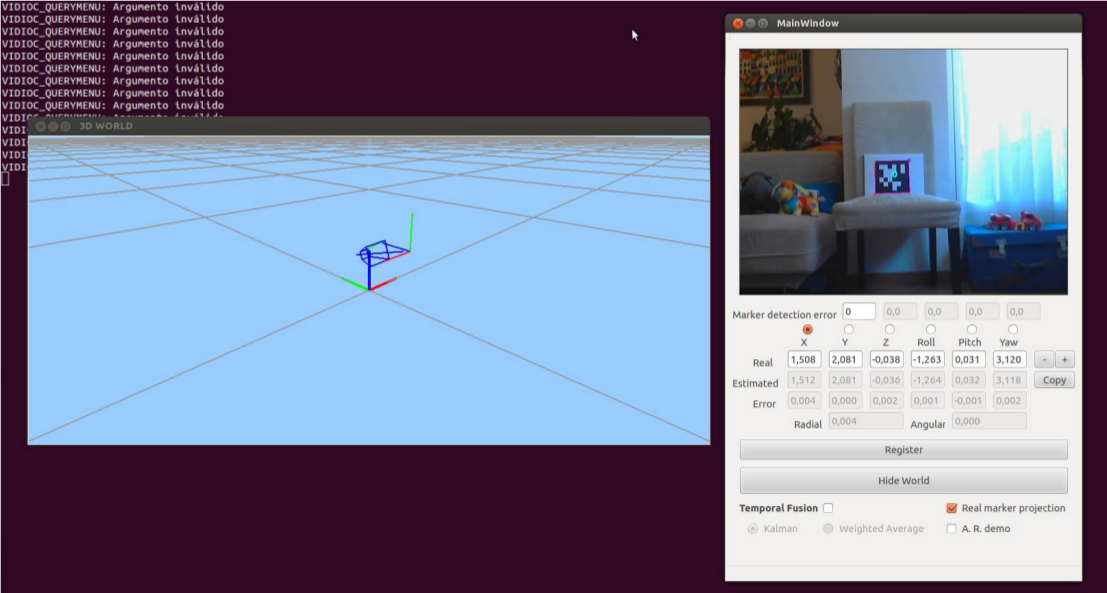
\includegraphics[scale=0.35]{Figures/cap-ceron.png}
\decoRule
\caption[Captura de pantalla, TFM de Alberto Lopéz-Cerón]{Captura de pantalla del componente desarrollado por Alberto Lopéz-Cerón.}
\label{fig:ceron}
\end{figure}

\newpage

En el proyecto fin de carrera de Daniel Martín Organista \parencite{ref5} se ha planteado un sistema de odometría visual, basado en sensores RGBD. El sistema desarrollado consta de algoritmos de estimación de la posición y trayectoria 3D de manera incremental en tiempo real, basándose en la información 3D ofrecida por el sensor RGBD. El sistema ha sido validado experimentalmente tanto en entornos reales como simulados (Figura~\ref{fig:dani}).

\begin{figure}[th]
\centering
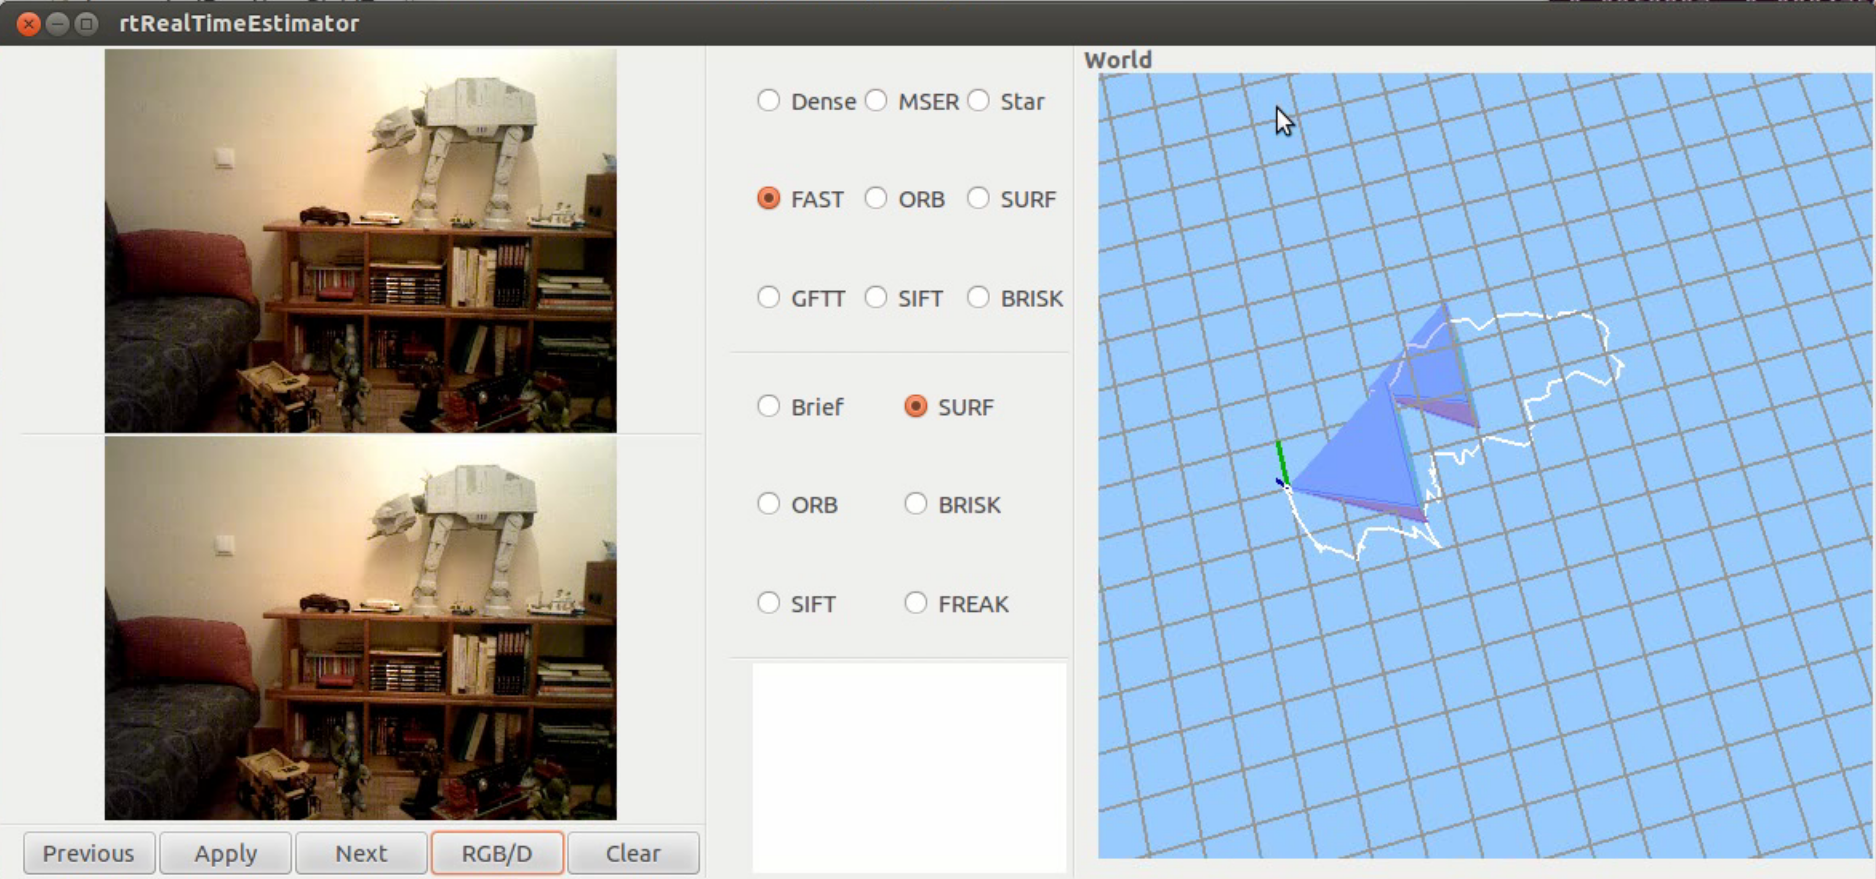
\includegraphics[scale=0.2]{Figures/cap-dani.png}
\decoRule
\caption[Captura de pantalla, PFC de Daniel Martín]{Captura de pantalla del componente desarrollado por Daniel Martín.}
\label{fig:dani}
\end{figure}

Por último, en el trabajo fin de master de Ignacio San Román Lana \parencite{ref4} se desarrolla un sistema clásico de odometría visual 3D en el que se emparejan puntos característicos entre fotogramas consecutivos o seguidos en el tiempo, para después optimizar un sistema de ecuaciones que estima la matriz fundamental. El resultado obtenido es mostrado en una ventana OpenGL en donde se puede ver la posición actual de la cámara y su recorrido.

El presente proyecto fin de carrera pretende unirse a los trabajos descritos en la búsqueda de algoritmos y técnicas de autolocalización visual, concretamente la odometría visual. En los próximos capítulos se detallará en la explicación de la solución adoptada.

El resto de la memoria consiste en 5 capítulos más:
\begin{itemize}
\item Objetivos - Se detallarán los objetivos del trabajo, así como la metodología llevada a cabo para la resolución del problema planteado.
\item Infraestructura - Se mostrarán las bases y técnologías empleadas.
\item Desarrollo - Se explicará el desarrollo del componente realizado y se detallarán tanto las bases teóricas como los algoritmos implementados.
\item Experimentos - Se muestran los experimentos realizados a fin de validar la solución optada.
\item Conclusiones - Se plantearán las conclusiones extraídas en base a los resultados obtenidos y se propondrán algunas líneas de trabajo futuras.

\end{itemize}
% Chapter Template

\chapter{Infraestructura} % Main chapter title

\label{Chapter3} % Change X to a consecutive number; for referencing this chapter elsewhere, use \ref{ChapterX}

En este capítulo se detallarán las herramientas base empleadas en la realización de este trabajo.

%----------------------------------------------------------------------------------------
%	SECTION Hardware
%----------------------------------------------------------------------------------------
%\section{Hardware}

%-----------------------------------
%	SUBSECTION Sensor
%-----------------------------------
\section{Sensores RGBD}

Los sensores RGBD son capaces de captar a parte de las componentes roja, verde y azul de la luz, información de profundidad (o "D"\ depth en inglés). Es decir, por cada píxel asocia la información de color con su correspondiente componente de profundidad. Esta tecnología fue desarrollada por la empresa israelí \textbf{PrimeSense}. El sensor Kinect dispone también de un micrófono multiarray con el cual puede predecir de dónde proviene el sonido.

En el 2010 Microsoft sacó al mercado el sensor Kinect (Figura~\ref{fig:Kinect}) para la consola de juegos Xbox 360 y Xbox One. Pronto se convirtió en uno de los dispositivos electrónicos más vendidos en todo el mundo después de su lanzamiento.

\begin{figure}[th]
\centering
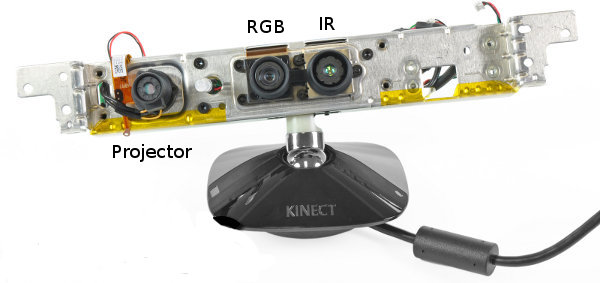
\includegraphics[scale=0.85]{Figures/ros_kinect.jpg}
\decoRule
\caption[Kinect sensor]{Sensor Microsoft Kinect}
\label{fig:Kinect}
\end{figure}

Este sensor salió al mercado a un precio mucho más reducido que algunos que existían antes que él por lo que el interés por este tipo de sensores se disparó y comenzaron a aparecen en diferentes áreas de la tecnología, como interfaces naturales de usuario (en inglés natural user interface, NUI), reconstrucción y realidad virtual o cartografía 3D.

El sensor utilizado en este trabajo es el \textbf{Asus Xtion PRO LIVE} que dispone de la misma tecnología comercializado por Asus, que proporciona profundidad, color y audio (utilizando un micrófono multiarray como el sensor Kinect). \footnote{https://www.asus.com/3D-Sensor/Xtion\_PRO\_LIVE/}

\begin{figure}[th]
\centering
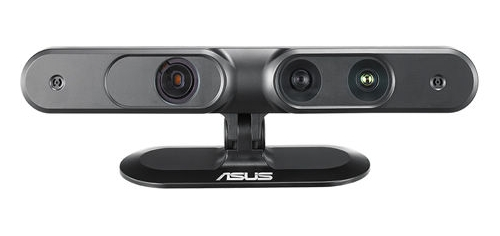
\includegraphics[scale=0.85]{Figures/xtion-pro-live.jpg}
\decoRule
\caption[Kinect sensor]{Asus Xtion PRO LIVE}
\label{fig:Kinect}
\end{figure}


\begin{table}
\caption{Especificaciones técnicas del Asus Xtion PRO LIVE}
\label{tab:xtion}
\centering
\begin{tabular}{ l | l }
\toprule
Campo de visión: & 58º H, 45º V, 70º D\\
\hline
Distancia de uso: & Entre 0.8m y 3.5m\\
\hline
Tamaño de la imagen de profundidad: & VGA (640x480) : 30 fps \\
				& QVGA (320x240): 60 fps\\
\hline
Resolución: & SXGA (1280*1024) \\
\bottomrule
\end{tabular}
\end{table}

Las especificaciones técnicas de este sensor se encuentran recogidas en la tabla ~\ref{tab:xtion}
%----------------------------------------------------------------------------------------
%	SECTION Software
%----------------------------------------------------------------------------------------
%\section{Software}

%-----------------------------------
%	SUBSECTION JDeRobot
%-----------------------------------
\section{JDeRobot}

JDeRobot es un proyecto desarrollado por el grupo de robótica de la Universidad Rey Juan Carlos \footnote{http://jderobot.org}. Consiste en una plataforma de desarrollo de aplicaciones robóticas y de visión artificial. Está en su mayoría escrito en C++, donde disponen de una colección de componentes capaces de comunicarse a través de ICE middleware \footnote{https://zeroc.com/products/ice}, los componentes pueden ejecutarse en diferentes ordenadores y pueden ser programados en diferentes lenguajes.

JdeRobot incluye numerosas herramientas, drivers, interfaces, librerías y tipos. Es \textit{software} libre con licencia GPL y LGPL. También utiliza \textit{software} de terceros como Gazebo, ROS, OpenGL, GTK y Eigen entre otros.

La versión de JdeRobot empleada ha sido la versión 5.4.0. A continuación se detallarán los componentes de JdeRobot que han sido de utilidad para la realización de este proyecto.

\subsection{Biblioteca Progeo}

Es una biblioteca de geometría proyectiva incluida en JdeRobot, que proporciona funciones muy útiles que relacionan puntos en dos y tres dimensiones.

Ha sido realmente útil en este trabajo para que a partir de puntos en dos dimensiones (píxeles) y su correspondiente información de profundidad (distancia), sacar los puntos relativos de la cámara en tres dimensiones.

Progeo usa el modelo de cámara \textbf{Pinhole}, en la Figura~\ref{fig:Pinhole} se puede observar la representación geométrica de la retroproyección y la proyección. Este modelo es definido por unos parámetros intrínsecos y extrínsecos que definen la composición de todos los parámetros iniciales de configuración de la cámara. Los parámetros extrínsecos que establecen la posición 3D, foco de atención (foa) y roll, mientras que los parámetros intrínsecos determinan la distancia focal y el centro óptico o píxel central.

\begin{figure}[th]
\centering
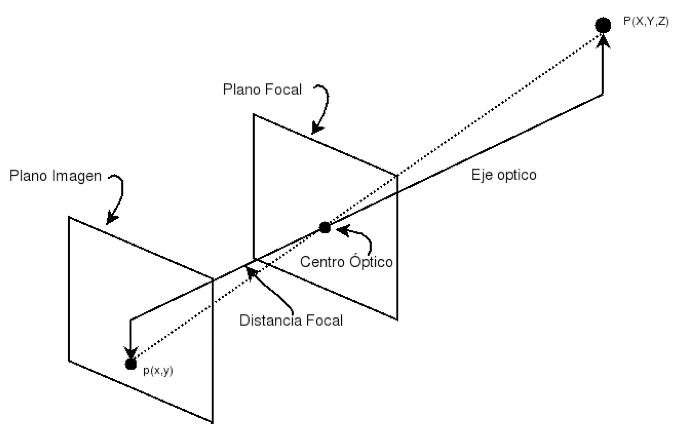
\includegraphics[scale=0.5]{Figures/pinhole-model.jpg}
\decoRule
\caption[pinhole]{Modelo de cámara Pinhole}
\label{fig:Pinhole}
\end{figure}

Las funciones que proporciona esta biblioteca son las siguientes:

\begin{itemize}
\item \textbf{Project}: Esta función permite proyectar un punto 3D del mundo al correspondiente pixel en 2D de la imagen de la cámara. 

\item \textbf{Backproject}: Esta función es capaz de a partir de las coordenadas de un píxel en 2D, obtener la línea de proyección que conecta la cámara y el foco con el rayo 3D que proyecta dicho píxel en el plano imagen. Con esto y conociendo la distancia real del punto 3D a calcular, se calcula las coordenas reales del punto 3D.

\item \textbf{DisplayLine}: Esta función permite conocer si una línea definida por dos puntos en 2D es visible dentro del plano imagen. 

\item \textbf{Display\_info}: Esta función muestra toda la información sobre la cámara utilizada.

\end{itemize}

\subsection{Biblioteca parallelIce}

Es otra librería incluída en JdeRobot, que soluciona el problema de latencia de información proveniente de los diferentes drivers, evitando la espera y proviniendo de un acceso asíncrono a una copia en local de las interfaces con muy bajo tiempo de procesado.

\subsection{Servidor OpenniServer}

OpenniServer es un driver que se comporta como un servidor y es capaz de proporcionar con un sensor RGBD (Kinect o Xtion), imágenes de color, de profundidad o nubes de puntos que son enviados a través de la interfaz ICE a un puerto específico, donde se pueden escuchar los datos. Este driver es el que se necesita para el funcionamiento de este trabajo ya que es desde donde se recogen tanto las imagenes de color (RGB) como las de profundidad (Depth) para su posterior procesado.

\subsection{Herramienta RGBDViewer}

Es una herramienta que permite enseñar la información proveniente de los sensores RGBD con openniServer como forma de visualización de los datos; imágenes RGB, DEPTH o nubes de puntos.

El funcionamiento corresponde a un hilo de ejecución llamado Control que se encarga de recolectar las imágenes provenientes del driver, una clase Shared para guardar y recoger los datos, y por último una clase Gui que se encargará de coger los datos (imágenes y nubes de puntos) guardados en Shared y mostrarlas.

%\begin{figure}[th]
%\centering
%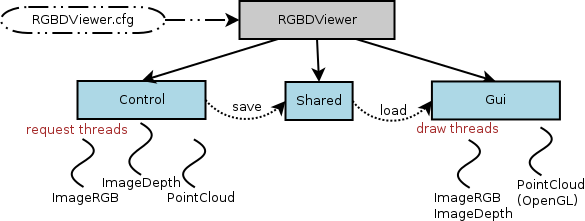
\includegraphics[scale=0.65]{Figures/rgbdviewer.png}
%\decoRule
%\caption[rgbdviewer]{Estructura del funcionamiento de RGBDViewer.}
%\label{fig:RgbdViewer}
%\end{figure}

Esta herramienta a servido como referencia para la realización de este trabajo. En la Figura~\ref{fig:RgbdViewer} podemos ver una captura de pantalla con las diferentes visualizaciones. 

\begin{figure}[th]
\centering
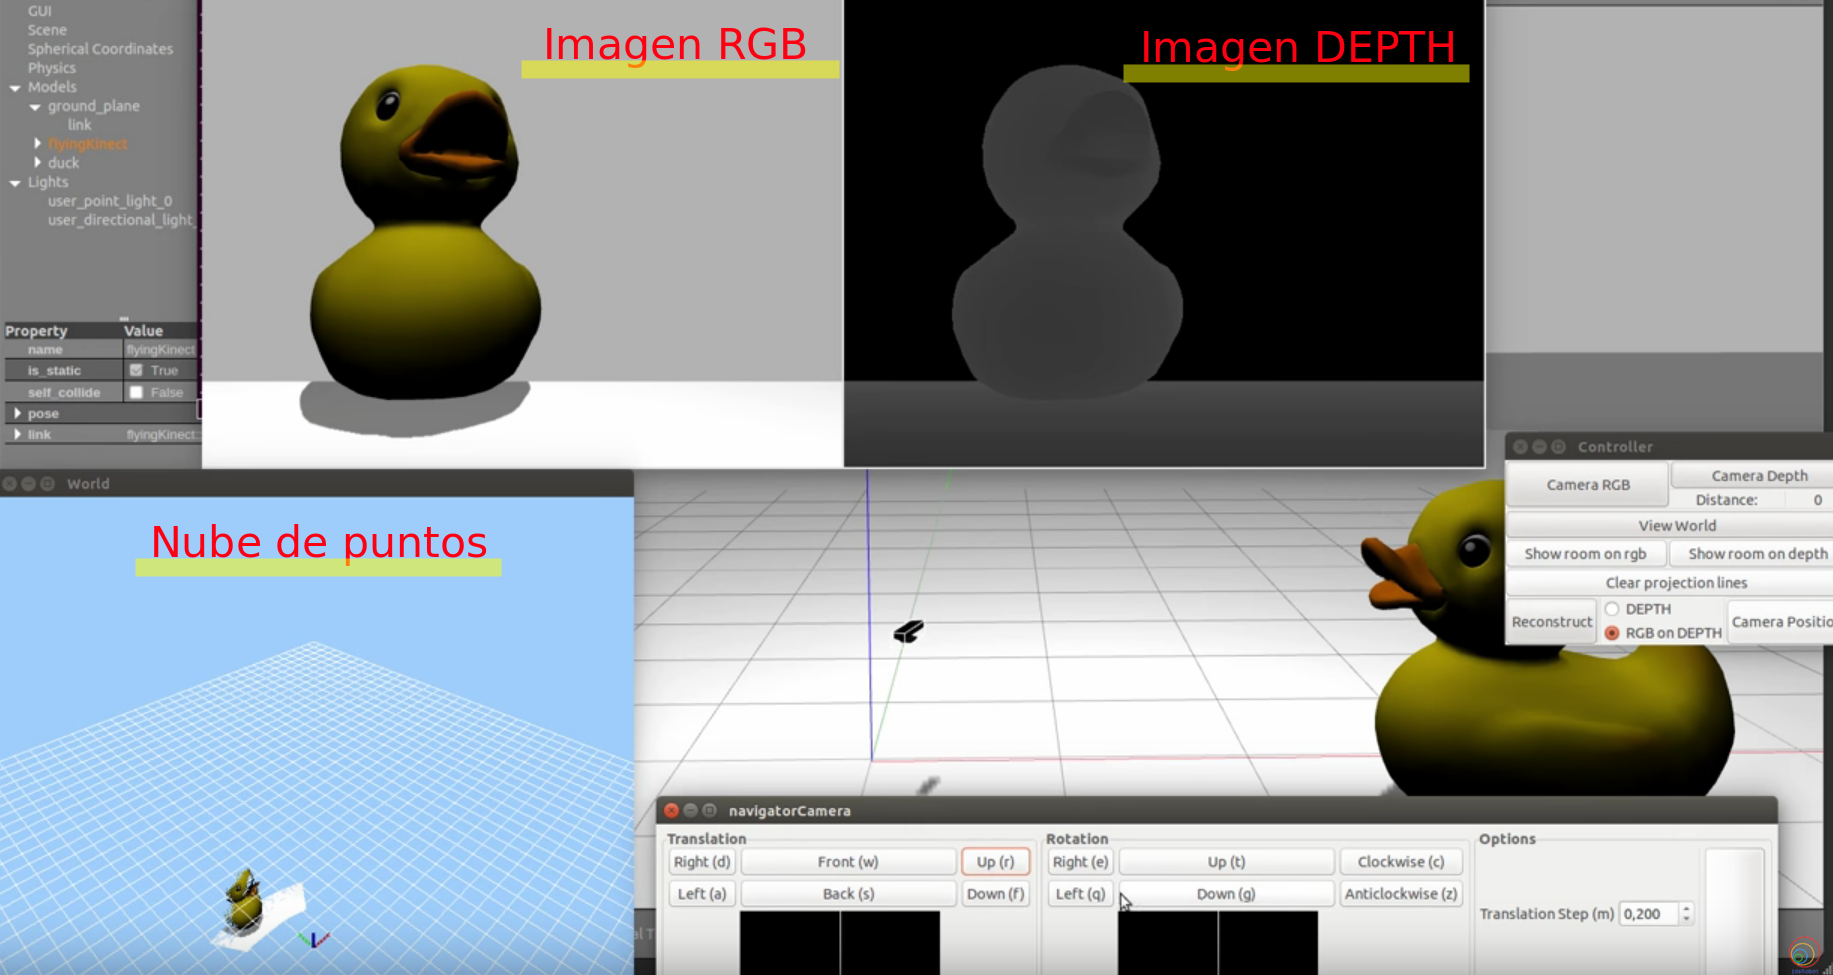
\includegraphics[scale=0.2]{Figures/rgbdviewer2.png}
\decoRule
\caption[rgbdviewer2]{Captura de pantalla del con las tres vistas de los diferentes datos, imagen de color, de profundidad y nube de puntos.}
\label{fig:RgbdViewer}
\end{figure}

\subsection{Pose3D}

Es una interfaz que define una posición en tres dimensiones (x, y, z, h) y una orientación con un cuaternión (q0, q1, q2, q3).

%\subsection{RGBPoint}

%Es una estructura de datos en la cual se pueden guardar puntos en tres dimensiones con coordenadas (x, y, z), color (r, g, b) y un identificador (id). 
%Para generar las nubes de puntos se ha usado un vector de esta estructura.

%-----------------------------------
%	SUBSECTION ICE
%-----------------------------------
\section{Biblioteca ICE de comunicaciones}

ICE (Internet Communications Engine) es un RPC framework desarrollado por ZeroC con soporte en C++, C\#, Java, JavaScript y Python entre otros. Se encuentra bajo doble licencia GNU GPL y código cerrado. Actúa como plataforma de comunicaciones y funciona bajo TCP/IP. \footnote{https://zeroc.com/products/ice}

En JdeRobot la podemos encontrar como librería y es utilizada como protocolo de comunicaciones entre los diferentes componentes de JdeRobot. En nuestro trabajo se ha usado la versión 3.5.1 y nos ha servido para establecer la comunicación entre el componente y el driver del sensor, recogiendo las imágenes de éste.

%-----------------------------------
%	SUBSECTION PCL
%-----------------------------------
\section{Biblioteca Point Cloud Library (PCL)}

PCL es una librería desarrollada en C++ para el procesamiento de imágenes 2D/3D y nubes de puntos. Está publicada con licencia BSD y libre bajo usos comerciales y de investicación. Está financialmente soportada por un consorcio de companías comerciales y su propia organización sin ánimo de lucro, \textbf{Open Perception}. A parte de los donadores y contribuidores individuales que aportan al proyecto. \footnote{http://pointclouds.org/}

Para simplificar el uso y el desarrollo, esta librería se encuentra dividida en módulos individuales de los que destacan el filtrado de puntos \textit{outliers} o de ruido, estructuras de datos, estimación 3D, algoritmos para la detección de puntos de interés, combinación, segmentación, algoritmos para el reconocimiento de objetos.
%En la Figura~\ref{fig:Grouping} se puede ver un ejemplo de reconicimiento de objetos basado en el módulo pcl\_recognition.

%\begin{figure}[th]
%\centering
%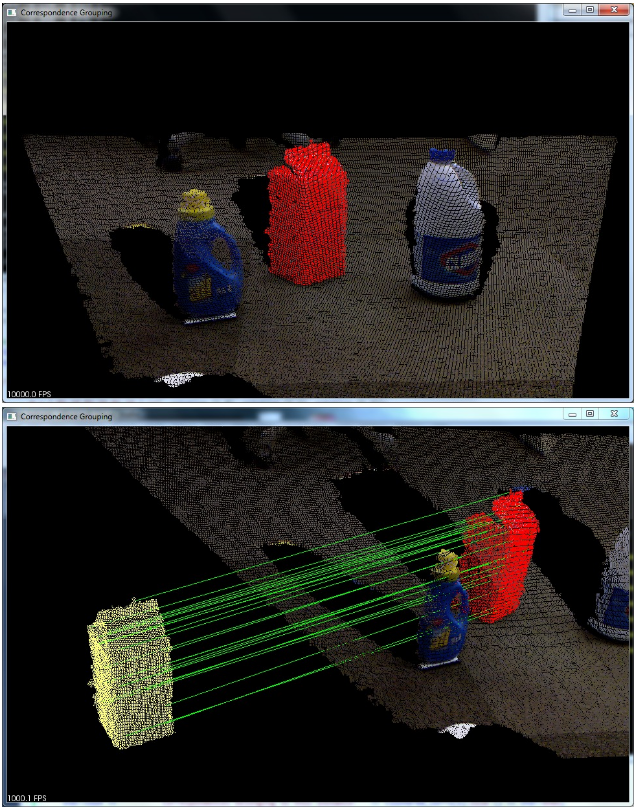
\includegraphics[scale=0.6]{Figures/correspondence_grouping.png}
%\decoRule
%\caption[grouping]{Reconocimiento de objeto 3D con PCL}
%\label{fig:Grouping}
%\end{figure}

En su página web disponen de mucha información y ejemplos prácticos que ayudan mucho a la compresión de todas las funcionalidades de esta librería. PCL también dispone de una librería i/o de entrada y salida para leer o crear nubes de puntos a partir de diferentes dispositivos, así como visualizadores 3D.


%-----------------------------------
%	SUBSECTION OpenCV
%-----------------------------------
\section{Biblioteca OpenCV}

OpenCV (Open Source Computer Vision Library) es una librería de código abierto que fue desarrollada para proporcionar una infraestructura común en aplicaciones de visión artificial y facilitar la inteligencia máquina, con mecanismos de aprendizaje y de interpretación de datos. Con licencia BSD da facilidades para su uso y su modificación bajo fines comerciales. \footnote{http://opencv.org/}

La librería contiene más de 2500 algoritmos. Estos algoritmos pueden ser usados para detectar y reconocer rostros, identificar objetos, clasificar acciones humanas determinadas en vídeos, seguimiento del movimiento de cámaras, seguimiento de objetos, extraer modelos de objetos 3D, producir nubes de puntos a partir de cámaras, encontrar imágenes similares de un conjunto, juntar trozos de imágenes para producir una imagen final con más resolución, etc... OpenCV tiene más de 47 miles de usuarios en la comunidad, excediendo los 14 millones de descargas, la librería es usada ampliamente en empresas, grupos de investigación y organismos gubernamentales.

OpenCV a sido diseñada de forma eficiente y con un fuerte enfoque en aplicaciones de tiempo real. Escrita en C/C++, la librería obtiene las ventajas del procesamiento multi-núcleo. Dispone de interfaces en C++, C, Python, Java y MATLAB y es soportada por diferentes sistemas operativos como Windows, Linux, Android y Mac OS.

En este trabajo se ha utilizado la versión 2.4.8 y se ha usado a la hora de identificar puntos de interés y para los distintos métodos de emparejamiento. En la Figura~\ref{fig:SiftDetector} se puede apreciar un ejemplo de su uso en la detección de puntos de interés sobre un entorno real.

\begin{figure}[th]
\centering
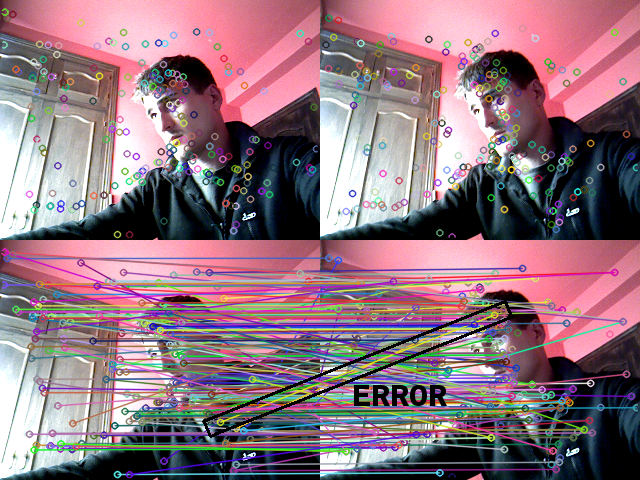
\includegraphics[scale=0.8]{Figures/sift-detector.png}
\decoRule
\caption[sift-detector]{Detección y emparejamiento de puntos de interés con OpenCV usando SIFT.}
\label{fig:SiftDetector}
\end{figure}

%-----------------------------------
%	SUBSECTION Eigen
%-----------------------------------
\section{Biblioteca Eigen}
Eigen es una librería de algebra lineal que permite hacer operaciones aritméticas con matrices y vectores, a través de los operadores comunes de C++, tales como +, -, * o a través de métodos especiales tales como dot(), cross(), etc... Para la clase \textit{Matrix} (matrices y vectores) los operadores solo soportan operaciones de álgebra lineal. En Figura~\ref{fig:Eigen} se puede ver un ejemplo de como de simple es hacer una multiplicación y una división por un escalar. \footnote{http://eigen.tuxfamily.org/}

\begin{figure}[th]
\centering
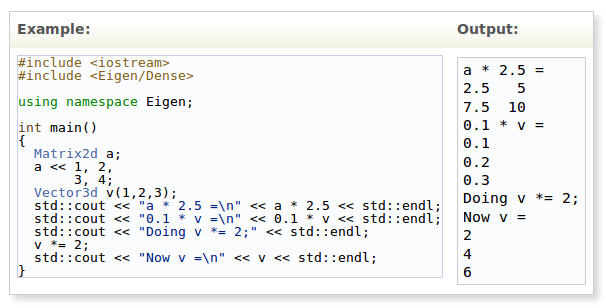
\includegraphics[scale=0.65]{Figures/eigen-multiplication.png}
\decoRule
\caption[eigen]{Ejemplo de una multiplicación y división por un escalar con Eigen.}
\label{fig:Eigen}
\end{figure}

Eigen es \textit{software} libre y desde la versión 3.1.1 tiene licencia MPL2 (LGPL3+ para las anteriores versiones). Se ha usado la versión 3.2.0 y ha sido de utilidad en este proyecto para realizar los cálculos de la matriz RT a través del los vectores de puntos 3D ya emparejados.

%-----------------------------------
%	SUBSECTION GTK
%-----------------------------------
\section{Biblioteca de interfaz gráfica GTK+}
GTK+, o the GIMP Toolkit es una herramienta multiplataforma de creación de interfaces gráficas. Es multiplataforma y está escrito en C, pero a sido diseñado para tener soporte para un gran rango de lenguajes, tales como Perl y Python. GTK++ tiene una gran colección de \textit{widgets} y interfaces para usar en la aplicación, tales como ventanas, botones, selectores, cajas de texto, etc.

La versión utilizada ha sido la 3.10.8. Es \textit{software} libre y parte del proyecto GNU. Con licencia LGPL, permite que sea utilizado por todos los desarrolladores, incluyendo aquellos que están desarrollando un  \textit{software} privativo. GTK+ ha sido utilizado en muchos proyectos y en grandes plataformas. \footnote{https://www.gtk.org/}

\subsection{Glade}
Glade es una \textit{RAD tool} (Rapid Application Development Tool) que permite desarrollar de manera fácil y rápida interfaces de usuario en GTK+ para el entorno de escritorio GNOME. La interfaz gráfica diseñada en Glade es guardada en un XML que usando los objetos GTK+ de \textbf{GtkBuilder} pueden ser cargados y utilizados por aplicaciones de forma dinámica como se ha hecho en este trabajo. \footnote{https://glade.gnome.org/}
%-----------------------------------
%	SUBSECTION OpenGL
%-----------------------------------
\section{OpenGL}
OpenGL es el principal entorno para el desarrollo de aplicaciones gráficas 2D y 3D interactivas. Desde 1992, OpenGL se ha convertido en la interfaz de aplicaciones gráficas más utilizada y soportada en la industria 2D y 3D, con miles de aplicaciones diponibles en diferentes plataformas. OpenGL ayuda al desarrollo de aplicaciones al incorporar un amplio conjunto de renderizado, mapeo de texturas, efectos especiales y otras potentes funciones de visualización. Se puede usar OpenGL en la mayoría de entornos de escritorio y diferentes plataformas. Es muy utilizada y conocida en la industria de los videojuegos.

Algunas de las ventajas de las que presume OpenGL son; que es un estándar de la industria, con soporte, multiplataforma y el único libre. Es estable, dispone de compatibilidad hacia atrás, escalable, fácil de usar y bien documentado. \footnote{https://www.opengl.org/}

Se ha usado la librería \textbf{Mesa 3D Graphics} en linux que es una implementación de la especificación de OpenGL con código abierto \footnote{https://www.mesa3d.org/}.

OpenGL en este trabajo se ha usado para visualizar la posición de la cámara, su estela y la colección de nubes de puntos obtenida y procesada de las imágenes RGB y de profundidad. En la Figura~\ref{fig:OpenGL} se puede apreciar una captura de pantalla con la posición de la cámara dibujada en el espacio tridimensional con el visualizador utilizado con OpenGL.

\begin{figure}[th]
\centering
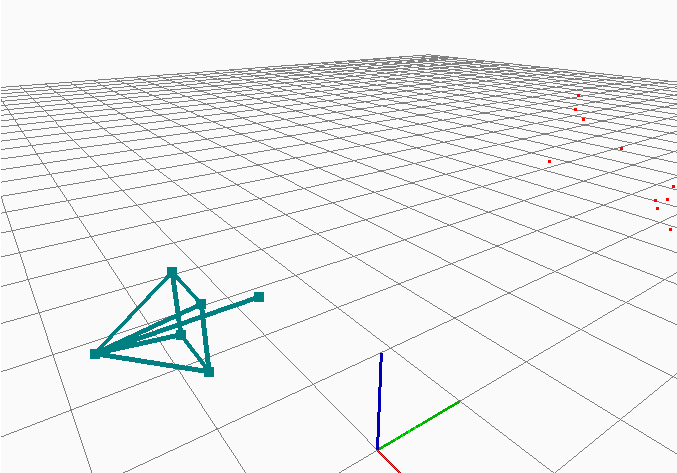
\includegraphics[scale=0.65]{Figures/camera-opengl.png}
\decoRule
\caption[opengl]{Captura de la posición de la cámara en el visualizador 3D con OpenGL.}
\label{fig:OpenGL}
\end{figure}
%\include{Chapters/Chapter2} 
%\include{Chapters/Chapter3}
%\include{Chapters/Chapter4} 
%\include{Chapters/Chapter5} 

%----------------------------------------------------------------------------------------
%	THESIS CONTENT - APPENDICES
%----------------------------------------------------------------------------------------


%----------------------------------------------------------------------------------------
%	BIBLIOGRAPHY
%----------------------------------------------------------------------------------------

\printbibliography
%[heading=bibintoc]

%----------------------------------------------------------------------------------------

\end{document}  
